\chapter{Being Hurt and Hurting Others}

This chapter follows J. Krishnamurti's dialogue with Dr. Alan W. Anderson on religion, attention, hurt, and education. There is no blackboard mathematics in the source video for this chapter, so the mathematical form here is deliberately schematic: it gives us a compact notation for the order of the inquiry, not a formal psychological model. The source remains the spoken inquiry: thought is not to be abolished; rather, we ask what thought can and cannot do, what attention is, and why psychological hurt prevents a mind from being whole.

\section{Religion Before Belief}

Anderson begins by protecting the inquiry from a crude conclusion. In the previous conversations, Krishnamurti has not said that thought must be destroyed, nor that knowledge is evil in itself. The question is subtler: what is the proper relation between thought, knowledge, intelligence, and that activity which religious traditions have tried to name as God?

Krishnamurti's first move is not to answer with doctrine. He says that words such as religion, love, and God have been so abused that they have nearly lost their meaning. Religion, as ordinarily practiced, has become superstition, propaganda, belief, ritual, and worship of images made either by the hand or by the mind. So before the conversation can proceed, the word religion has to be cleaned of its inherited burden.

We can write the false map in a compact form:
\begin{equation}
\text{religion}_{\text{common}}
\Rightarrow
\text{belief}+\text{ritual}+\text{fear}+\text{image}+\text{authority}.
\end{equation}
This is not Krishnamurti's definition of religion. It is the structure he is rejecting. The word has become tied to systems of belonging and consolation, and therefore to thought's need for security.

The correction is equally compact:
\begin{equation}
\text{religion}_{\text{inquiry}}
\Rightarrow
\text{gathering of total energy}.
\end{equation}
This is the first important turn. Religion is not a set of beliefs about an object called God. It is the gathering of energy at every level--physical, moral, and inward--so that there is attention.

\subsection{Question \& Answer}

\paragraph{Question.}
If thought is not to be abolished, why can it not be the instrument that reaches the religious or the immeasurable?

\paragraph{Answer.}
Because in this dialogue thought is described as conditioned, fragmentary, never new, and never free. Thought has its necessary place, but it cannot capture what is beyond its own measure. The task is not to attack thought, but to see its limit.

In schematic form:
\begin{equation}
\text{thought}
\Rightarrow
\text{conditioned}+\text{fragmentary}+\text{not new}+\text{not free}.
\end{equation}
The next movement of the lecture follows from this limit. If thought cannot capture the immeasurable, then one must ask what quality of mind can meet it.

\section{Gathering Energy Into Attention}

Krishnamurti gives a precise working meaning to religion: the gathering together of all energy, which brings about great attention. In that attention, he says, there is no frontier. This is the axis of the first half of the conversation.

We should not read this as a technique. He is not recommending concentration exercises or an inward discipline built around reward. He is setting up a distinction between the mechanical action of thought and the quality of attention in which thought is understood.

\begin{definition}
In this chapter, \emph{attention} means the gathering of the whole energy of the human being--brain, mind, heart, nerves, and perception--without exclusion, resistance, effort, frontier, or expectation.
\end{definition}

A useful reconstruction of the spoken structure is:
\begin{align}
\text{gathering of energy}
&\Rightarrow \text{attention},\\
\text{attention without frontier}
&\Rightarrow \text{perception beyond the measure of thought}.
\end{align}

The word ``beyond'' must be handled carefully. It does not mean romantic belief, speculation, or sentimentality. Krishnamurti explicitly rejects all of those. It means that the movement of thought, being conditioned and fragmentary, cannot possess the whole.

\begin{figure}
\centering
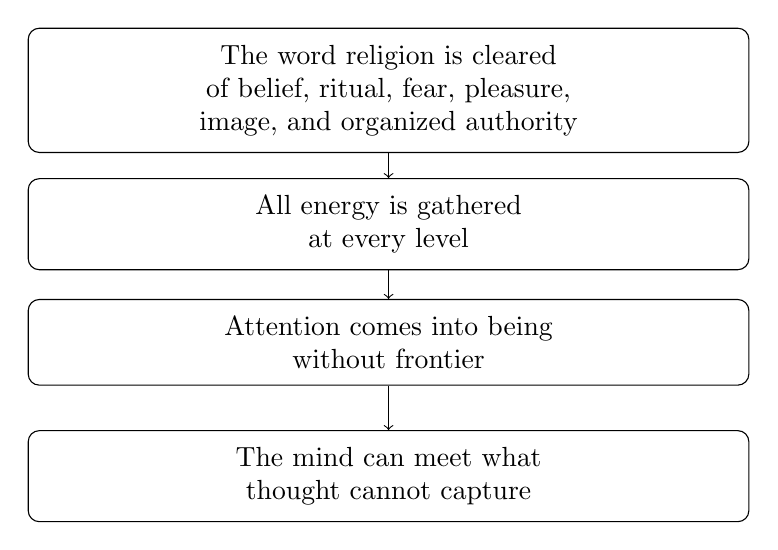
\begin{tikzpicture}
\node[draw, rounded corners, text width=.72\linewidth, align=center, inner sep=6pt] (a) at (0,0)
{The word religion is cleared\\of belief, ritual, fear, pleasure,\\image, and organized authority};
\node[draw, rounded corners, text width=.72\linewidth, align=center, inner sep=6pt] (b) at (0,-1.7)
{All energy is gathered\\at every level};
\node[draw, rounded corners, text width=.72\linewidth, align=center, inner sep=6pt] (c) at (0,-3.2)
{Attention comes into being\\without frontier};
\node[draw, rounded corners, text width=.72\linewidth, align=center, inner sep=6pt] (d) at (0,-4.9)
{The mind can meet what\\thought cannot capture};
\draw[->] (a) -- (b);
\draw[->] (b) -- (c);
\draw[->] (c) -- (d);
\end{tikzpicture}
\caption{A transcript-based reconstruction of the opening movement: religion is redefined as gathered energy becoming attention.}
\end{figure}

This figure is not a blackboard reproduction. It is a compact map of the spoken inquiry.

\section{The Priest, Fear, and the Loss of Nature}

Anderson brings in biblical language about stillness and the inadequacy of human thought to reach the divine. Krishnamurti responds by shifting the scale from scripture to the history of religious mediation. When human beings lost touch with nature--with clouds, birds, lakes, the earth, and the beauty of direct perception--the priest entered.

The priest becomes mediator between the human and the so-called divine. He interprets, explains, commands, and exploits. What was simple becomes mixed up. What was direct becomes mediated. What was the adoration of beauty becomes fear and propaganda.

The structure is not accidental. It can be set down as a chain:
\begin{equation}
\text{loss of contact with nature}
\Rightarrow
\text{mediation}
\Rightarrow
\text{authority}
\Rightarrow
\text{fear}.
\end{equation}

This is also why the chapter belongs to the larger architecture of false maps of happiness. The priest offers more than the daily routine of bread, house, work, desire, and death. He appears to offer the goods: security, grace, continuity, preservation. But this security is purchased at the cost of fear.

Krishnamurti then returns to the earlier definition. If religion is the gathering of energy into total attention, then organized fear is not religion. The measurable and mechanical have their place, but when life becomes merely mechanical, another reaction appears: superstition, gurus, rituals, and promises of spiritual safety.

\section{The Religious Mind and the Quiet Mind}

The lecture now moves from public religion to the quality of mind. Krishnamurti asks what kind of mind can perceive something beyond the measurement of thought. The question is repeated because it is not rhetorical. It is the center of the inquiry.

A mind that can perceive must be quiet. This quietness is not induced silence, nor withdrawal, nor obedience. It is the simple fact that if the mind is chattering, it does not listen. If it is occupied with itself, it cannot attend.

We can express the local logic as a short derivation.

\begin{proposition}
Within this dialogue, quietness is not a decorative spiritual state; it is a condition of perception.
\end{proposition}

\begin{proof}
First, perception requires listening and seeing. Second, a mind occupied with its own movement does not listen or see directly. Third, the chattering movement of thought occupies the mind with itself. Therefore, for perception to be direct, the mind must be quiet. This is not a technique for becoming quiet; it is the recognition that in noise, attention is absent.
\end{proof}

Anderson then tests the language of devotion and one-pointedness. Krishnamurti immediately asks whether attention is one-pointed. The question matters because one-pointedness can easily become focus, and focus can become exclusion.

\subsection{Question \& Answer}

\paragraph{Question.}
Is attention one-pointed?

\paragraph{Answer.}
Not if one-pointedness means concentration on an object. Anderson clarifies that he meant integration rather than focus, but Krishnamurti's question exposes a danger. If attention is made into a point, it may become concentration, and concentration excludes.

The distinction is sharp enough to deserve a table.

\begin{table}
\centering
\begin{tabular}{|p{.42\linewidth}|p{.42\linewidth}|}
\hline
\textbf{Concentration} & \textbf{Attention} \\
\hline
Brings thought to a point & Gives the whole energy of being \\
\hline
Excludes what is not selected & Does not exclude \\
\hline
Builds a barrier around focus & Has no frontier \\
\hline
Involves effort and resistance & Has no resistance and no effort \\
\hline
Can strengthen division & Sees division and duality \\
\hline
\end{tabular}
\caption{A transcript-based contrast between concentration and attention.}
\end{table}

The same test is applied to receptivity and waiting. If we say the mind is receptive, Krishnamurti asks who is there to receive. If we say the mind waits, then there is one who waits and something expected. Again duality enters. The lecture proceeds by removing these hidden divisions.

\section{Why Human Beings Are Hurt}

At this point Krishnamurti gathers the earlier themes. A mind that is attentive has understood relationship and responsibility, has understood psychological fear, and has understood the movement of pleasure. Then comes the next question: what is such a mind? The answer is not abstract. It requires looking at hurt.

He distinguishes physical pain from psychological hurt. Physical pain can be watched; it need not corrode the whole quality of mind. Psychological hurt is more difficult because it enters the structure of the self. A hurt mind is not innocent, and this lack of innocence prevents total attention.

\begin{definition}
\emph{Psychological hurt}, in this chapter, means the wound sustained by the image one has of oneself. It is not merely physical pain, and it is not merely the thought that one has been hurt.
\end{definition}

Anderson proposes that hurt may arise when one starts thinking about thinking that one is hurt. Krishnamurti says it is deeper. From childhood, the child is compared with another child. That comparison is already the beginning of hurt.

The local sequence can be written:
\begin{align}
\text{comparison}
&\Rightarrow \text{image of oneself},\\
\text{image of oneself}
&\Rightarrow \text{resistance wall},\\
\text{resistance wall touched}
&\Rightarrow \text{hurt}.
\end{align}

This is not a formal law. It is a careful shorthand for the movement Krishnamurti describes. The image is a wall between you and me. When that wall is touched at its tender point, I am hurt.

\subsection{Question \& Answer}

\paragraph{Question.}
Is hurt simply a matter of thinking about the fact that one has been hurt?

\paragraph{Answer.}
No. The lecture says the matter is deeper. Hurt begins with comparison, imitation, and the building of an image. Thought may sustain and repeat the hurt, but the vulnerable structure is the image itself.

One can see this by a small worked example, using only the lecture's own categories.

\paragraph{Worked example.}
Suppose a child is told, ``Your brother is clever; you are not.'' The sequence is not merely that the child hears a sentence. The sentence introduces comparison. Comparison invites an image: ``I am the inferior one.'' That image becomes a point of resistance. Later, another casual word touches the same image, and the hurt repeats.

In schematic form:
\begin{equation}
\text{comparison: ``he is clever, I am not''}
\Rightarrow
\text{self-image}
\Rightarrow
\text{woundable identity}.
\end{equation}

The same structure appears with name, body, class, status, nationality, family, and tradition. A name by itself is not the problem. ``Mr. Brown'' is only a name. The problem begins when thought builds an image around the name: superior, inferior, ancient family, respectable class, Brahmin, non-Brahmin, aristocrat, success, failure.

\begin{equation}
\text{name}+\text{body}+\text{status}+\text{tradition}
\Rightarrow
\text{image sustained by thought}.
\end{equation}

Krishnamurti's point about the word and the thing enters here. If one sees that the word is not the thing and the description is not the described, then the sacredness of a name, even the name of God, loses its psychological power. The danger is not sound or spelling; it is identification.

\section{Healing Hurt Without Making a Method}

The lecture then raises two questions with unusual clarity. Can the hurts already received be healed so that not a mark is left? And can future hurt be prevented completely, without resistance, withdrawal, or escape?

These are not two separate topics. They are two sides of the same inquiry:
\begin{align}
Q_1 &: \text{Can past hurt end without leaving a mark?}\\
Q_2 &: \text{Can future hurt not be added?}
\end{align}
The notation \(Q_1,Q_2\) is only a label for the two spoken questions.

Anderson suggests that complete attention might dissolve the image. Krishnamurti agrees only after making a crucial correction. We cannot use attention as a means to wipe away hurt. That would turn attention into a method, and method belongs to the old mechanical movement.

\subsection{Question \& Answer}

\paragraph{Question.}
Can attention be used as a tool to wipe away hurt?

\paragraph{Answer.}
No. The order is the reverse. One must understand the image, hurt, education, family, and society in which the image was formed. Out of that understanding comes attention. If I am hurt and simply try to apply attention as a remedy, I am still acting from hurt.

The corrected order is:
\begin{equation}
\text{understanding hurt}
\Rightarrow
\text{attention},
\qquad
\text{not}
\qquad
\text{attention as technique}
\Rightarrow
\text{erasure of hurt}.
\end{equation}

This is one of the most important safeguards in the chapter. The inquiry must not become a program. Krishnamurti asks us to look at hurt, not translate it, not wish to wipe it away, not escape it, but see it. The seeing includes insults, negligence, casual words, gestures, and the language that wounds.

From hurt, a series of reactions follows:
\begin{equation}
\text{hurt}
\Rightarrow
\text{violence}+\text{fear}+\text{withdrawal}+\text{search for safety}.
\end{equation}
The search for safety may even create an idea of God as one who will never hurt. Here the beginning of the lecture returns: religion made by fear is not religion; it is a projection of hurt.

\section{Education as the Act of Love}

The last movement translates the inquiry into education. Anderson raises the case of a child who arrives at school already hurt. Krishnamurti says that the child is already hurt, and hurt because it is hurt. From hurt come violence, fear, withdrawal, neurotic action, and acceptance of anything that promises safety.

The usual response is to continue the structure that produced the hurt. The parent compares. The school gives marks. The teacher transmits information. Society praises imitation. Even religion says, ``Be like Krishna, Buddha, or Jesus.'' Krishnamurti says this too is hurt.

The educational problem is therefore not secondary. It is the concrete test of the inquiry:
\begin{equation}
\text{hurt parent}+\text{hurt teacher}+\text{hurt child}
\Rightarrow
\text{civilization continues hurt}.
\end{equation}

But another relation is possible. When the educator realizes that he is hurt and that the child is hurt, the relationship changes. In the very act of teaching, whether the subject is mathematics or anything else, he is freeing himself from hurt and helping the child be free of hurt.

\begin{figure}
\centering
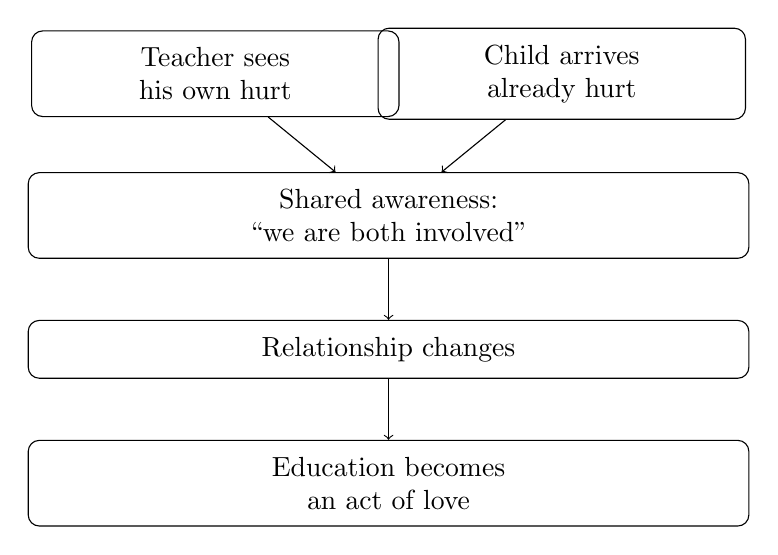
\begin{tikzpicture}
\node[draw, rounded corners, text width=.35\linewidth, align=center, inner sep=6pt] (t) at (-2.2,0)
{Teacher sees\\his own hurt};
\node[draw, rounded corners, text width=.35\linewidth, align=center, inner sep=6pt] (c) at (2.2,0)
{Child arrives\\already hurt};
\node[draw, rounded corners, text width=.72\linewidth, align=center, inner sep=6pt] (s) at (0,-1.8)
{Shared awareness:\\``we are both involved''};
\node[draw, rounded corners, text width=.72\linewidth, align=center, inner sep=6pt] (r) at (0,-3.5)
{Relationship changes};
\node[draw, rounded corners, text width=.72\linewidth, align=center, inner sep=6pt] (l) at (0,-5.2)
{Education becomes\\an act of love};
\draw[->] (t) -- (s);
\draw[->] (c) -- (s);
\draw[->] (s) -- (r);
\draw[->] (r) -- (l);
\end{tikzpicture}
\caption{A transcript-based reconstruction of the educational relation: hurt is not solved by information, but by shared seeing in relationship.}
\end{figure}

The teacher does not begin with a subject alone. He begins by seeing what hurt does: it kills, destroys, produces violence, and makes one want to hurt others. Only then can teaching become relationship rather than transmission.

The final complication is Anderson's question about whether a hurt person will misinterpret the activity of one who is not hurt. Krishnamurti's answer is stark: there are very few who are not hurt-bound. He says, humbly but directly, that many things have happened to him and yet he does not know what it means to be hurt. Whether or not the reader can say this, the point for education is clear: it is possible not to add hurt.

At the end Anderson asks whether they might next take up the relationship of love to all this. Krishnamurti agrees. The chapter closes there because the word love has now been prepared. It is not sentiment. It is not coercion. In this lecture it first appears as the act in which teacher and child see hurt together and help each other be free of it.

\section{Summary}

The movement of the chapter is a single arc. Thought is not denied, but its limit is seen. Religion is not belief or ritual, but the gathering of total energy into attention. Attention is not concentration, receptivity, waiting, or method. It has no exclusion, resistance, effort, or frontier.

The obstacle to such attention is psychological hurt. Hurt is not merely the idea that one has been hurt; it is rooted in comparison, imitation, self-image, name, status, and identification. The image becomes a wall, and when the wall is touched, the person is wounded.

The lecture's final question is educational and relational. Can past hurt be healed without a mark, and can future hurt end without resistance? The answer is not a method. It begins in understanding hurt directly. In education, that means the teacher and child see together that both are hurt. When that seeing changes relationship, Krishnamurti calls it an act of love.